\documentclass[tikz,border=10pt]{standalone}
\usetikzlibrary{calc}
\begin{document}
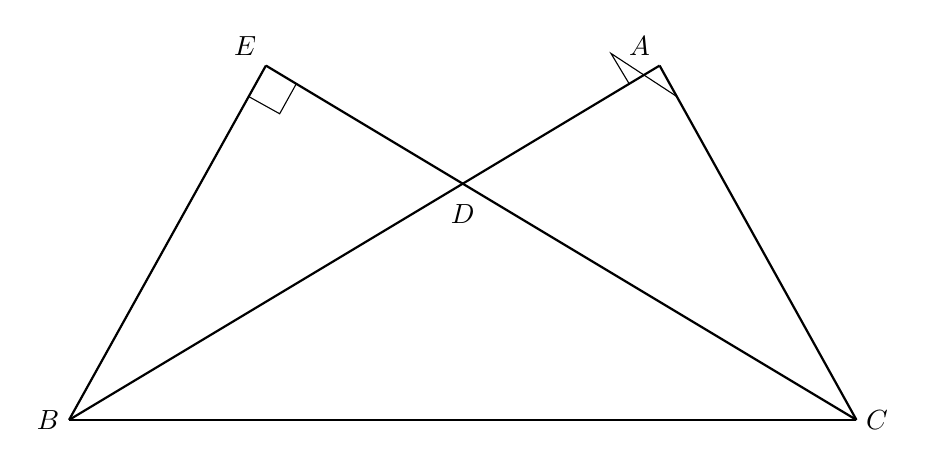
\begin{tikzpicture}[scale=1]
  \coordinate (B) at (0,0);
  \coordinate (C) at (10,0);
  \coordinate (A) at (7.5,4.5);
  \coordinate (E) at (2.5,4.5);
  \coordinate (D) at (intersection of B--A and E--C);

  \draw[thick] (B) -- (A);
  \draw[thick] (E) -- (C);
  \draw[thick] (B) -- (E);
  \draw[thick] (A) -- (C);
  \draw[thick] (B) -- (C);

  % right-angle mark at A
  \draw ($(A)!0.45cm!(B)$) -- ($($(A)!0.45cm!(B)$)!0.45cm!90:(A)$) -- ($(A)!0.45cm!(C)$);
  % right-angle mark at E
  \draw ($(E)!0.45cm!(B)$) -- ($($(E)!0.45cm!(B)$)!0.45cm!-90:(E)$) -- ($(E)!0.45cm!(C)$);

  \node[above left] at (A) {$A$};
  \node[above left] at (E) {$E$};
  \node[left] at (B) {$B$};
  \node[right] at (C) {$C$};
  \node[below=4pt] at (D) {$D$};
\end{tikzpicture}
\end{document}
